% ===================================================================
% Presentación con Latex Beamer -> EN proceso de modificación -> CCF
% ===================================================================
\documentclass[9pt,xcolor=svgnames]{beamer}
%\documentclass[handout,xcolor=svgnames]{beamer} %Version imprimible
% -------------------------------------------------------------------
\usepackage{paquetes}
\usepackage{licencia}
% -------------------------------------------------------------------
\usepackage{modo}
% -------------------------------------------------------------------

% Comienza el documento
\begin{document}
% Tikz -> Imágenes
\tikzstyle{every picture}+=[remember picture]
% Entorno matemático
\everymath{\displaystyle}

% Transparencia de Inicio -> Título
\begin{frame}
  \titlepage
\end{frame}

\normalsize

% Transparencia de índice
\begin{frame}
 \frametitle{Índice} 
 %\transboxin
 \tableofcontents
\end{frame}

\section{Introducción}
\section{Motivación}

\paragraph{}
Mi interés por el mundo de los videojuegos, desde muy pequeño, y tras haber cursado en la carrera
la asignatura optativa de "Diseño de videojuegos", donde aprendí mucho
relacionado con el desarrollo de estos,
aumentó mi interés por este mundo y además el desarrollo de ellos. Por lo que desde entonces consideraba seriamente realizar 
como proyecto fin de carrera un videojuego.

\paragraph{}
También he de añadir que tras conocer abiertamente el mundo del Software libre, gracias a la importancia que se le presta
en la Universidad de Cádiz. Se decidió que el proyecto fuera software libre bajo licencia GPL 3. Y así cualquier persona
interesada en el desarrollo de videojuegos y en el software libre en general, pudiera usar los recursos del proyecto
libremente.

\section{Objetivos}

\paragraph{}
El objetivo del proyecto es realizar un videojuego de conducción en dos dimensiones con vista cenital\footnote{Los elementos son
vistos desde arriba}. Se podría decir que el juego tendrá tintes de juegos como Micro Machines, disponible para diversas 
plataformas, y del Mario Kart de Nintendo. En el siguiente capítulo se explica más detalladamente el objetivo 
concreto del proyecto.

\paragraph{}
Otro de los objetivos principales del proyecto, es la realización del juego tanto para personas que
dedican varias horas a la consecución de videojuegos, tanto para personas casuales, que dedican poco tiempo
jugando. Por lo que ser un juego de conducción el cual no esta compuesto por ninguna historia o trama argumental, facilita que se 
le pueda dedicar pequeños intervalos de tiempo o, sin embargo, dedicarle varias horas al día.

\paragraph{}
Otro de los objetivos del proyecto, es poder hacerlo ampliable, de forma que cualquier persona mediante indicaciones y manuales
pueda añadir tanto nuevos personajes, como circuitos en los que competir.

\section{Estructura del documento}

\paragraph{}
Este documento esta compuesto por las siguientes partes:

\begin{itemize}
    \item \textbf{Introducción}: pequeña descripción del proyecto, así como los objetivos y estructura del documento.
    
    \item \textbf{Descripción general}: descripción más amplia sobre el proyecto, así como todas las características relevantes
    que tendrá.
    
    \item \textbf{Planificación}: exposición de la planificación del proyecto y las distintas etapas que esta compuesto el mismo.
    
    \item \textbf{Análisis}: fase de análisis del sistema, empleando la metodología seleccionada. Se definirán los
    requisitos funcionales del sistema, diagramas de caso de uso, diagramas de secuencia y contrato de las operaciones.

    \item \textbf{Diseño}: realización del diseño del sistema, diagramas de secuencia y clases aplicadas al diseño.
    
    \item \textbf{Implementación}: aspectos más relevantes durante la implementación del proyecto. Y problemas que han aparecido 
    durante el desarrollo de este.
    
    \item \textbf{Pruebas y validaciones}: pruebas realizada a la aplicación, con el fin de comprobar su correcto funcionamiento y
    cumplimiento de las expectativas.
    
    \item \textbf{Conclusiones}: conclusiones obtenidas tras el desarrollo de la aplicación.
    
    \item \textbf{Apéndices}: 
    \begin{itemize}
        \item \textbf{Herramientas utilizadas}: explicación de todas las herramientas usadas a lo largo del desarrollo del 
        proyecto.
        \item \textbf{Manual de instalación}: manual para la correcta instalación del proyecto en el sistema.
        \item \textbf{Manual de usuario}: manual de usuario para el correcto uso de la aplicación.
        \item \textbf{Manual de para añadir nuevos personajes}: manual donde se explica los distintos pasos necesarios para añadir
        nuevos personajes al juego.
        \item \textbf{Manual de para añadir nuevos circuitos}: manual donde se explica los distintos pasos necesarios para añadir
        nuevos circuitos al juego.
    \end{itemize}
    
    \item \textbf{Bibliografía}: libros y referencias consultado durante el desarrollo del proyecto.
    
    \item \textbf{Licencia GPL 3}: texto completo sobre la licencia GPL 3, por la cual se rige el proyecto.

\end{itemize}


\section{Descripción}

\section{Descripción}

\paragraph{}
El proyecto consiste en un juego de carreras en dos dimensiones con vista cenital, en el que se podrá competir contra 
coches dirigidos por el ordenador. La idea es realizar un juego entretenido y dinámico, que estará compuesto por varios modos de juego.

\begin{figure}[H]
  \label{logo_zycars}
  \begin{center}
    
\includegraphics[scale=0.5]{imagenes/logo_zycars.png}
  \end{center}
  \caption{Descripción: Logo de Zycars}
\end{figure}

\section{Características del videojuego}

\paragraph{}
El videojuego ofrece una alternativa libre, gratuita y original para jugar a un juego de conducción en dos dimensiones. 
Las posibilidades que ofrece son las siguientes:

\subsection{Modos de juego}

\paragraph{}
En \emph{Zycars} tendremos distintos modos de juegos, en cada uno de ellos el
objetivo que habrá que llevar a cabo será distinto.
A continuación se describirán los distintos modos de juegos que tendrá el videjuego:

\subsubsection{Carrera rápida} 

\paragraph{}
El juego en el modo de carrera rápida ofrece la posibilidad de enfrentarnos a 3 personajes 
controlados por la inteligencia artificial, a lo largo de un circuito que
hayamos seleccionado previamente. El número de vueltas
que se realicen durante la carrera estarán a elección del jugador y se podrá elegir el número de las mismas a la hora de seleccionar
el circuito.

\subsubsection{Campeonato} 

\paragraph{}
En este modo de juego podremos competir contra 3 personaje dirigidos por el ordenador
a lo largo de un campeonato completo, el cual habremos elegido previamente. 

\paragraph{}
El campeonato estará compuesto por cuatro circuitos y el número de vueltas a estos, también estarán a elección del jugador 
al igual que en el modo de juego explicado anteriormente.

\paragraph{}
Tras la conclusión de cada una de las carreras, los jugadores obtendrán una puntuación en función de la posición que haya 
obtenido. El jugador que mayor puntuación haya conseguido tras acabar los cuatro circuitos, se proclamará ganador del 
campeonato.

\subsubsection{Contrarreloj} 

\paragraph{}
En este último modo de juego y a diferencia de los dos anteriores, el jugador competirá solo sin ningún oponente.

\paragraph{}
El objetivo en este modo de juego será la realización de los circuitos ofrecidos y mejorar los tiempos de estos, ya sean la 
vuelta más rápida del circuito o el tiempo general. El número de vueltas que deberemos dar al circuito serán un total de tres, a
diferencia de los modos anteriores, no tendremos la posibilidad de modificar el valor.

\subsection{Elementos de juego}

\paragraph{}
En esta sección se hará una pequeña descripción de los distintos elementos que encontraremos a lo largo del juego, ya sean 
manipulados por los jugadores, o encontrados a lo largo de los circuitos.

\subsubsection{Personajes}
	
\paragraph{}
Los elementos básico del juego, habrá disponibles distintos personajes que tendrán asociado un 
vehículo característico a su personalidad y apariencia. Cada uno de ellos
tendrán distintas características, 
cosa a tener en cuenta a la hora de hacer nuestra elección por uno de ellos, como la velocidad, la aceleración y el giro.
	
\begin{figure}[H]
	\label{ejemplo_personaje2}
	\begin{center}
		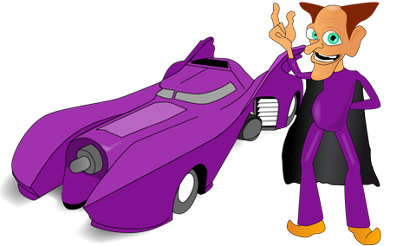
\includegraphics[scale=0.7]{imagenes/ejemplo_personaje2.png}
	\end{center}
	\caption{Descripción: Personaje de Zycars.}
\end{figure}

\subsubsection{Cajas de ítems} 

\paragraph{}
A lo largo de los circuitos en los que estemos compitiendo contra la inteligencia artificial, 
podremos encontrar distintas cajas que al colisionar con ellas nos proporcionen
aleatoriamente una habilidad o ítem que nos
ayuden en la competición contra nuestros rivales.

\begin{figure}[H]
	\label{item_box}
	\begin{center}
		
\includegraphics[scale=1]{imagenes/items/item_box.png}
	\end{center}
	\caption{Descripción: Caja de ítem.}
\end{figure}

\subsubsection{Tipos de ítems}

Los ítems que podremos obtener a partir de la caja de ítems, los podremos diferenciar principalmente en tres tipos:

\begin{description}
	\item \textbf{Ataques a distancia} Estos nos permitirán lanzar ataques
        de forma que podamos interceptar a los competidores que 
	se encuentres lejos de nosotros.
	
	\item \textbf{Obstáculos} Estos nos permitan dejar obstáculos en el
        recorrido, que reduzcan nuestra velocidad considerablemente
	o aquellos que al pasar por encima perdamos completamente el control de nuestro vehículo por unos instantes de tiempo.
	
	\item \textbf{Velocidad} Estos nos darán la opción de aumentar nuestra velocidad durante un pequeño intervalo de tiempo.
\end{description}

\section{Colaboradores}

\paragraph{}
Todo el apartado del proyecto referente a la programación del mismo se ha realizado de forma individual. En cambio, otros apartados
como el diseño gráfico, se ha contado con la colaboración de otra persona, y la música se ha obtenido de Internet, concretamente 
de Jamendo, la página de música libre publicadas bajo licencias Creative Commons. Los créditos de juego son los siguientes:

\begin{description}
    \item [Desarrollador] José J. Marente Florín
    \item [Diseñador Gráfico] David Nieto Rojas
    \item [Música] Bob Wizman, Pirato Ketchup, Los Cadaver, The Wavers, Zamalska 
\end{description}


\section{Calendario}
%\begin{frame}
    %\frametitle{Planificación}

      %  \begin{block}{Propuesta del PFC}
     %       A finales de Mayo del 2010 se comenzó a plantear que se podía realizar como proyecto fin de carrera. 
    %        Tuvo lugar las reuniones con el tutor, con el fin de obtener distintas ideas. Finalmente entre todas las ideas
   %         propuestas se decidió realizar este proyecto.
  %      \end{block}
 %       
%\end{frame}

\begin{frame}
    \frametitle{Planificación}

        \begin{block}{Tiempo de desarrollo}
            De septiembre de 2010 a septiembre de 2011.
        \end{block}
    
        \begin{block}{Fases}
        Durante el periodo de desarrollo tuvieron lugar las distintas fases:
            \begin{itemize}
                \item \textbf{Fase de análisis}: indentificación de las necesidades del software
                \item \textbf{Fase de diseño}: diseño de todo el sistema
                \item \textbf{Fase de aprendizaje}: familiarización con el lenguaje python y la biblioteca pygame
                \item \textbf{Fase de desarrollo}: implementación de todo los obtenido en la fase de diseño. Fase más larga
                \item \textbf{Pruebas y correcciones}: pruebas necesarias para comprobar el correcto funcionamiento. En paralelo a
                la fase de desarrollo
                \item \textbf{Redacción de la memoria}: realización de la memoria final
            \end{itemize}
        \end{block}

\end{frame}

\begin{frame}
    \frametitle{Diagrama de Gantt I}

        \begin{center}
                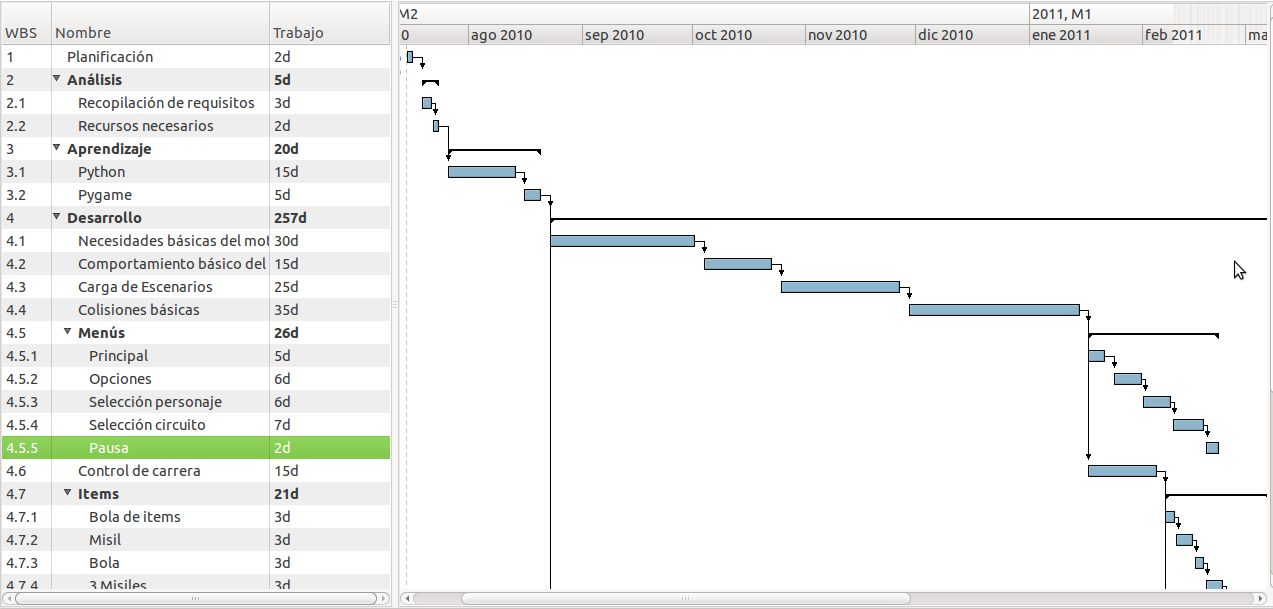
\includegraphics[scale=0.25]{imagenes/gant1.png}
        \end{center}
\end{frame}

\begin{frame}
    \frametitle{Diagrama de Gantt II}
        \begin{center}
                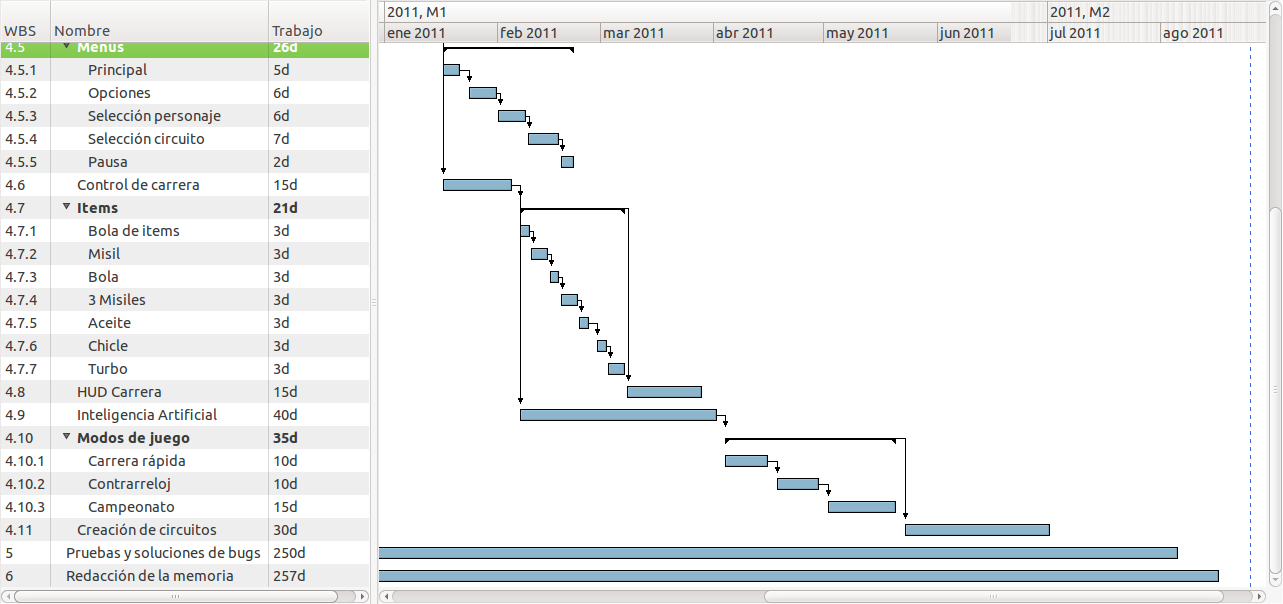
\includegraphics[scale=0.25]{imagenes/gant2.png}
        \end{center}
\end{frame}


\section{Implementación}
\begin{frame}
    \frametitle{Separar datos del código}

        %En todo momento se ha procurado separar todos los datos de los personajes, circuitos y menús, del código
        %fuente.\\
        Desacople código / datos (personajes, circuitos, menús, etc).\\
        \begin{block}{Ventajas}
            \begin{itemize}
                \item No es necesario saber programar para realizar cambios sobre cualquier parámetro
                \item Cualquier persona puede ampliar el juego con nuevos personajes y nuevos circuitos, siguiendo
                los manuales creados para ello
            \end{itemize}
        \end{block}
        \begin{block}{Solución}
            \begin{itemize}
                \item Todo se lee de ficheros XML
            \end{itemize}
        \end{block}

        \begin{center}
                
\includegraphics[scale=0.25]{imagenes/logo_xml.png}
        \end{center}

\end{frame}

\begin{frame}
    \frametitle{Formato de circuitos}

    \begin{block}{Mapas de tiles}
        Tile: imagen cuadrada usada para generar imágenes de mayor complejidad.\\
        Usor del editor de mapas Tiled.
    \end{block}   
    
    %\begin{block}{Editor de mapas: Tiled}
    %Proporcionaba todas las necesidades básicas, 
    %como una sencilla edición y creación de niveles, así como la gestión de capas,
    %para poder poner elementos en el circuito a un nivel superior o inferior.\\
    %Para ello se debía crear una imagen con todos los tiles que compondrían un circuito (tileset).\\
    %Genera como resultado un XML.
    %\end{block}   

        \begin{center}
                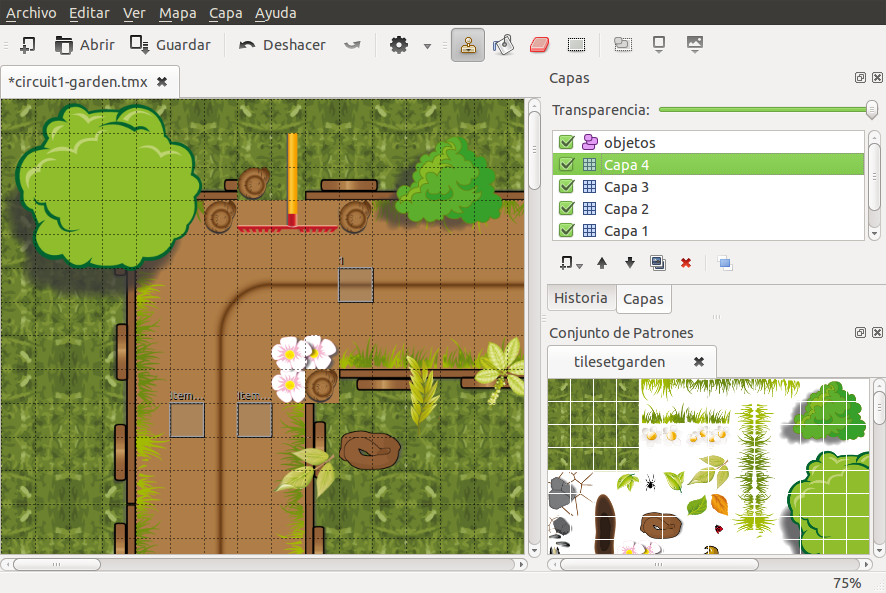
\includegraphics[scale=0.28]{imagenes/captura_tiled.png}
        \end{center}


\end{frame}

\begin{frame}
    \frametitle{Formato de circuitos}

    \begin{columns}

        \column{150px}

        \begin{block}{Inconveniente}
            %No permite indicar de forma sencilla que tiles eran atravesables, colisionables o de cualquier otro tipo.
            No permite indicar los tipos de los tiles.
        \end{block}
    
        \begin{block}{Solución}
        %Una imagen extra con las mismas características, donde los tiles sera de un único color, en función del tipo
        %que estos sean.
        Usar una imagen extra.
        \end{block}

        \column{180px}
        \begin{center}
                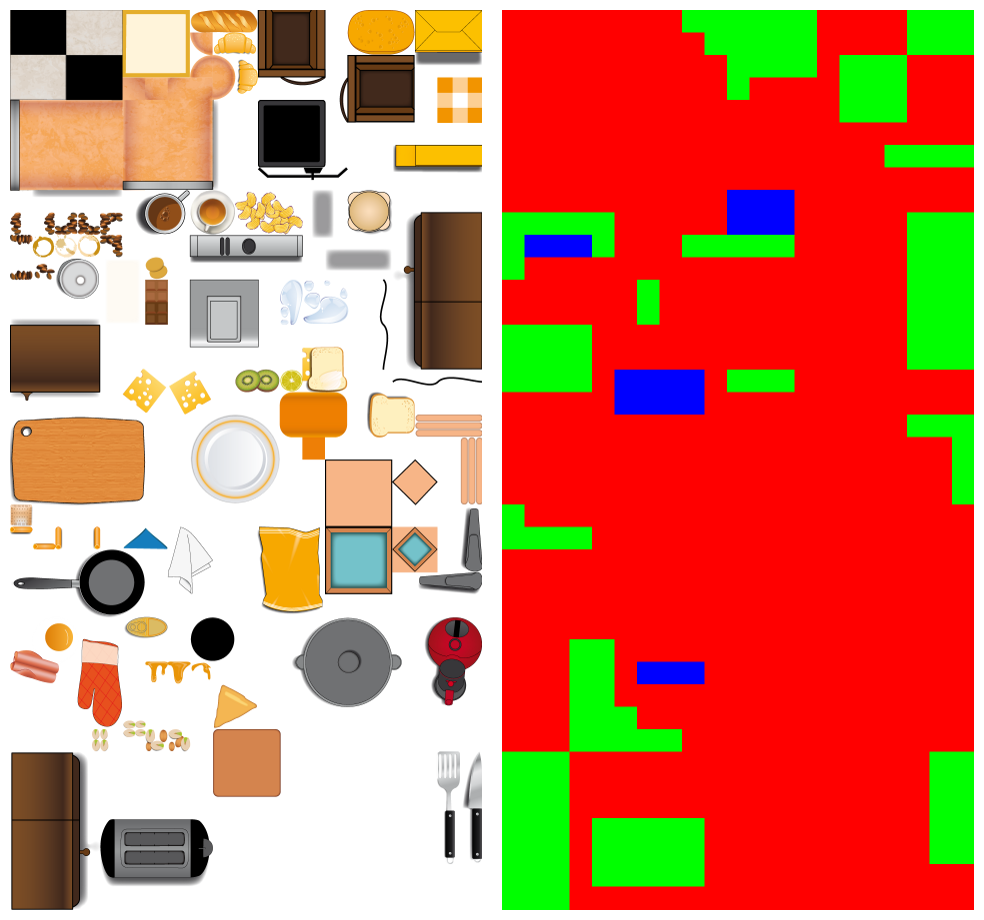
\includegraphics[scale=0.18]{imagenes/tileset-collisionmap.png}
        \end{center}
        
    \end{columns}

\end{frame}

\begin{frame}
    \frametitle{Colisiones}
    
    Una de los aspectos más importantes en este tipo de juegos.
    \begin{block}{Colisión con el escenario}
        \begin{itemize}
            \item Detectamos si atravesamos algún tile no atravesable
            \item Si es así corregimos la posición del coche en según la dirección, sentido y lado del tile por
            el que colisione
            \item En el caso de que el tile sea de tipo ralentizador, diminuimos la velocidad del coche
        \end{itemize}
    \end{block}

    \begin{center}
        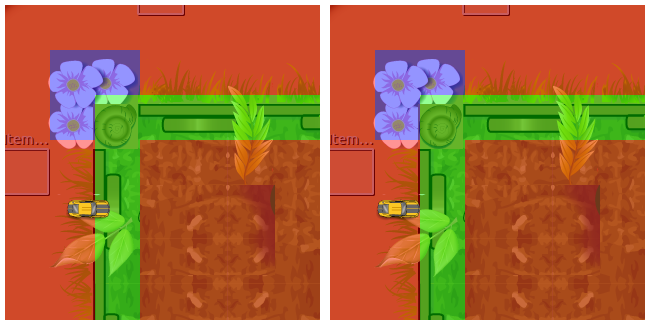
\includegraphics[scale=0.3]{imagenes/colision1-colision2.png}
    \end{center}
\end{frame}

\begin{frame}
    \frametitle{Colisiones}
    
    \begin{block}{Colisión entre vehículos}
        \begin{itemize}
            \item De forma similar a la colisión con el escenario
            \item Cuando se detecta la colisión se corrige la posición de los vehículos, en función la dirección, 
            sentido y lado por el que colisionen
            \item Podemos usar nuestro coche para evitar adelantamientos
        \end{itemize}
    \end{block}
    
    \begin{block}{Colisión con ítems de ataque}
      \begin{itemize}
            \item Se destruye el ítem y se cambia el estado del coche que colisiona
        \end{itemize}
    \end{block}
    
    \begin{block}{Colisión con obstáculos}
      \begin{itemize}
            \item Cambia el estado del coche en función del tipo de obstáculo (atravesable o no)
        \end{itemize}
    \end{block}

\end{frame}

\begin{frame}
    \frametitle{Inteligencia artificial}
    %Otro de los aspectos más importante de un videojuego de las características de Zycars, es la
    %inteligencia artificial, ya que en dos de los tres modos de juegos disponibles el objetivo es obtener la
    %mejor clasificación posible, por delante de los demás coches controlados por el ordenador
    Aspectos muy importante en videojuego de las características
    de Zycars: interviene en en dos de los tres modos de
    juegos.

        \begin{block}{Habilidades}
            \begin{itemize}
                \item Realización del recorrido: debe ser capaz de realizar los 
                recorridos de los circuitos
                \item Lanzamiento de ítems: también debe poder usar los ítems que reciba de las bolas de ítems
            \end{itemize}
        \end{block}
        
        \begin{center}
                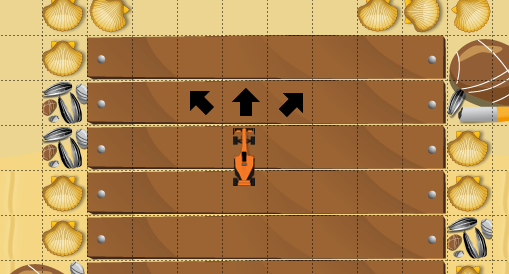
\includegraphics[scale=0.5]{imagenes/ia2.png}
        \end{center}
        

        
\end{frame}

\begin{frame}
    \frametitle{Realización del recorrido. Algoritmo A*}

    %Aprovechando que tenemos un circuito creado por tiles y que podemos saber en todo momento en el tile 
    %actual que se puede encontrar cualquiera de los competidores, se decidió implementar el 
    %algoritmo de búsqueda A*.
    
    Teniendo un circuito de tiles podemos realizar búsquedas de caminos a través de estos.

        \begin{block}{Objetivo}
        Buscar el camino más corto y óptimo desde
        un nodo origen, hasta un nodo destino. Se tienen en cuenta factores
        como el valor heurístico de los nodos, así como el coste real del recorrido.
        \end{block}

        \begin{block}{Parámetros}
        Los parámetros que se tienen en cuenta en la búsqueda:
            \begin{itemize}
                \item h’(n) es el valor heurístico del nodo actual n, hasta el final
                \item g(n) el coste real del camino desde el origen al nodo actual
                \item Función de evaluación: f(n) = g(n) + h’(n)
            \end{itemize}
        \end{block}

        \begin{block}{Estructuras}
            \begin{itemize}
                \item Lista de abiertos: nodos por los que aún no se han pasado
                \item Lista de cerrados: nodos por los que ya se han pasado
            \end{itemize}
        \end{block}
        
\end{frame}

\begin{frame}
    \frametitle{Realización del recorrido. Algoritmo A*}

    %\begin{columns}
    
        %\column{200px}
        \begin{block}{Funcionamiento}
            Partiendo del nodo actual:
            \begin{enumerate}
                \item Obtenemos vecinos
                \item Si no están en abiertos ni cerrados y los metemos en abiertos
                %\item Si alguno esta en abiertos, comprobamos su f(n), si es menor lo sustituiremos
                %\item Introducimos en abiertos los que cumplan las condiciones
                \item Obtenemos de abiertos el nodo con menor f(n) y comenzamos de nuevo 
                \item Una vez en el nodo objetivo, detenemos la búsqueda y devolvemos el camino
            \end{enumerate}
        \end{block}
        
        %\column{150px}
        \begin{center}
                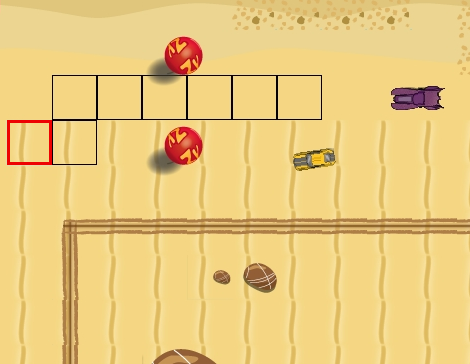
\includegraphics[scale=0.3]{imagenes/a*_ejemplo.png}
        \end{center}
    
    %\end{columns}

\end{frame}

\begin{frame}
    \frametitle{Lanzamientos de ítems}

    Capaz de lanzar los ítems disponibles a los largo del juego, según las
    distintas situaciones en la que se encuentre.

        \begin{block}{Solución}
        Cada vehículo tiene dos segmentos:
            \begin{itemize}
                \item Delantero: comprueba si algún oponente está delante para lanzar ítem
                \item Trasero: verifica la parte trasera en busca de algún oponente para dejar un obstáculo
            \end{itemize}
        %uno desde el centro delcoche hacia unos píxeles por delante su posición y otro desde el centro uno píxeles atrás de la posición.
        \end{block}

        \begin{center}
                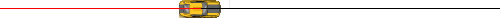
\includegraphics[scale=0.5]{imagenes/ia_segmentos.png}
        \end{center}

        \begin{center}
                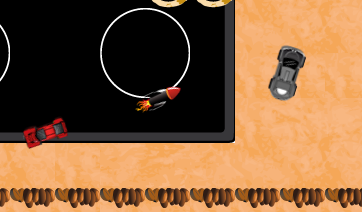
\includegraphics[scale=0.5]{imagenes/ia_lanzar.png}
        \end{center}
\end{frame}

\begin{frame}
    \frametitle{Recopilación}

    \begin{columns}
    
        \column{200px}
        \begin{block}{Zycars}
            \begin{itemize}
                \item Multiplataforma
                \item 12 circuitos
                \item 3 modos de juego
                \item 3 campeonatos
                \item 7 personajes
                \item 6 ítems
                \item Circuitos ampliables con tiled
                \item Personajes ampliables
                %\item Dificultad adecuada
            \end{itemize}
        %uno desde el centro delcoche hacia unos píxeles por delante su posición y otro desde el centro uno píxeles atrás de la posición.
        \end{block}

        \column{100px}
        \begin{center}
                
\includegraphics[scale=0.5]{imagenes/character2.png}
        \end{center}
    
    \end{columns}
        
\end{frame}


\section{Herramientas}
\begin{frame}
    \frametitle{Herramientas}

    \begin{columns}
    
        \column{200px}
        \begin{block}{Lenguaje de programación: Python}
        %Oportunidad perfecta para aprender un nuevo lenguaje de programación.\\
        Entre sus principales características:
            \begin{itemize}
                \item Sintaxis limpia y que favorece un código legible.
                \item Multiplataforma
            \end{itemize}
        %Destacar que se han obtenido unos resultado muy satisfactorios y ha cumplido todas las expectativas esperadas.

        \end{block}
        
        \column{100px}

        \begin{center}
                
\includegraphics[scale=0.22]{imagenes/logo_python.png}
        \end{center}
        
    \end{columns}

    \begin{columns}
    
        \column{200px}

        \begin{block}{Biblioteca gráfica: Pygame}
        %Wrapper de la biblioteca SDL, de C/C++, para Python, por lo que tiene todas las virtudes de dicha biblioteca:
        Conjunto de módulos de Python para la creación de videojuegos:
            \begin{itemize}
                \item Multiplataforma %compatible con Microsoft Windows, GNU/Linux, Mac OS y QNX
                \item Muy completa (imágenes 2D, sonido, música y entrada estándar)
                %\item Usada durante la asignatura de Diseño de Videojuegos, características conocidas.
            \end{itemize}
        \end{block}
        
        \column{100px}

        \begin{center}
                
\includegraphics[scale=0.24]{imagenes/logo_pygame.png}
        \end{center}
        
    \end{columns}

\end{frame}

\begin{frame}
    \frametitle{Herramientas}

        \begin{block}{Analizador de código: Pylint}
        Analiza el código Python en busca de errores y señales de mala calidad.\\
        La nota obtenida en el código del proyecto es de 8.25 sobre 10.
        \end{block}

        %\begin{block}{Sistema de control de versiones: Subversion}
        \begin{block}{Forja del proyecto}
        Alojado en el sistema que proporciona Google Code, bajo el sistema de control de versiones subversion.
            \begin{itemize}
                \item Pública
                \item Descargas para windows, linux y código fuente
                \item Página inicial (vídeos de demos, descripción, capturas, etc)
            \end{itemize}
        \end{block}

        \begin{block}{Documentación del código: Doxygen}
            \begin{itemize}
                \item Permite la documentación sencilla y legible de todo el código
                \item Generando en varios formatos como puede ser HTML o PDF
            \end{itemize}
        Para python existe la herramienta Doxypy.
        %que nos permite usar la convención de comentarios de Python y adaptarlos a Doxygen.
        \end{block}

\end{frame}



\section{Conclusiones}
\begin{frame}
    \frametitle{Conclusiones}

        \begin{block}{Cumplimiento de objetivos}
            \begin{itemize}
                \item Todos los objetivos marcados al inicio del PFC han sido cumplidos.
                \item Más duración de la esperada
                \item Contribución al mundo del software libre
                \item Juego de coches en 2D totalmente funcional
            \end{itemize}
        \end{block}

        \begin{block}{Valoración personal}
            \begin{itemize}
                \item Enfrentamiento a un proyecto complejo en solitario
                \item Aprendizaje de nuevas herramientas
                \item Puesta en práctica de conocimientos adquiridos
            \end{itemize}
        \end{block}


        \begin{block}{Posibles mejoras y ampliaciones:}
            \begin{itemize}
                \item Modo dos jugadores (pantalla dividida, juego en red)
                
                \item Soporte para varias resoluciones
                %cómodo para personas con pantalla muy pequeñas, como usuarios de netbooks, o también para persona con grandes resoluciones que desean una ventana de juego mayor.
                
                \item Grabación de las mejores vueltas
            \end{itemize}
        \end{block}
        
\end{frame}

\begin{frame}
    \frametitle{Conclusiones}
    \begin{center}
        {\huge Zycars se incluirá en la próxima versión de}\\
        \begin{center}
            {\Huge Guadalinex}
        \end{center}
    \end{center}

        
    \begin{columns}
    
        \column{100px}
        \begin{center}
            
\includegraphics[scale=0.4]{imagenes/andatuz.png}
        \end{center}
        
        \column{200px}
        \begin{center}
            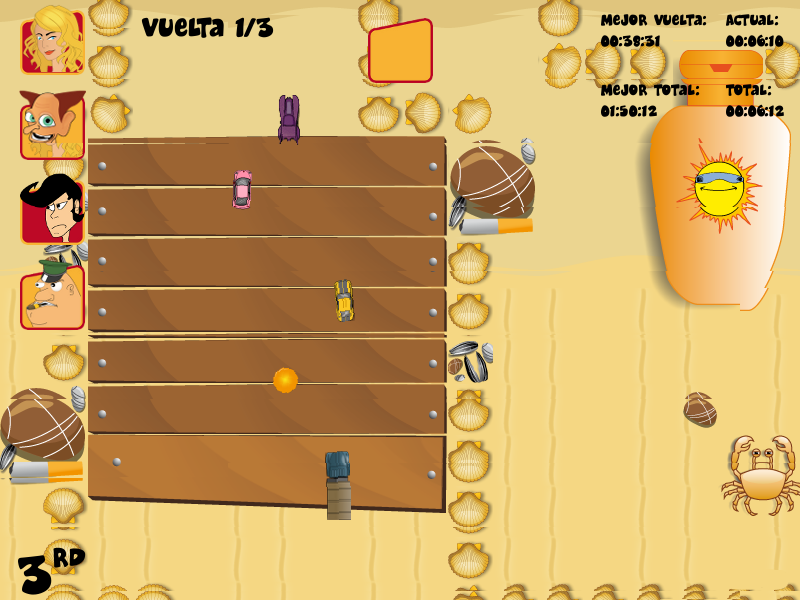
\includegraphics[scale=0.22]{imagenes/pantalla_juego.png}
        \end{center}
    \end{columns}

\end{frame}



%\section{Mejoras y ampliaciones}
%\input{contenido/mejoras.tex}

\section{Bibliografía}
\begin{frame}
    \frametitle{Bibliografía recomendada}
    \begin{thebibliography}{5}
        \beamertemplatearticlebibitems
            \bibitem{Python}	
            Página de \emph{Python}
            \newblock http://www.python.org/
            
            \bibitem{PyGTK}
            Página oficial sobre \emph{Pygame}
            \newblock http://www.pygame.org/
             
        \beamertemplatebookbibitems
            \bibitem{UML}
            Larman, Craig
            \newblock Applying UML and Patterns, 3ª Edición. Prentice Hall, 2004.
            
            \bibitem{Dive into Python}
            Pilgrim, Mark
            \newblock Dive into Python. Appress, 2004.
    \end{thebibliography}
\end{frame}

\begin{frame}
    \frametitle{Demostración}
    
    \begin{center}
        {\Huge Demostración de Zycars}
    \end{center}
    
    \begin{center}
        
\includegraphics[scale=0.4]{imagenes/logo_zycars.png}
    \end{center}

\end{frame}

\begin{frame}
    \frametitle{Esto es todo}
    
    \begin{center}
        {\Huge Gracias por su atención}\\
        \bigskip
        {\huge ¿Preguntas?}\\
        \bigskip
        {\LARGE http://code.google.com/p/zycars/}
    \end{center}

\end{frame}


%\section{Preguntas}

\end{document}
  
